\documentclass[../../../main.tex]{subfiles}

\begin{document}

\subsubsection{Real Space}

This lattice is also a triangular Bravais-lattice, only now with unit cell doubling (in the direction of $\vec{t}_2$), hence the unit cell has 6 sites. The Wigner-Seitz cell is a stretched hexagon. In the cartoon a different unit cell is shown.

\begin{center}
	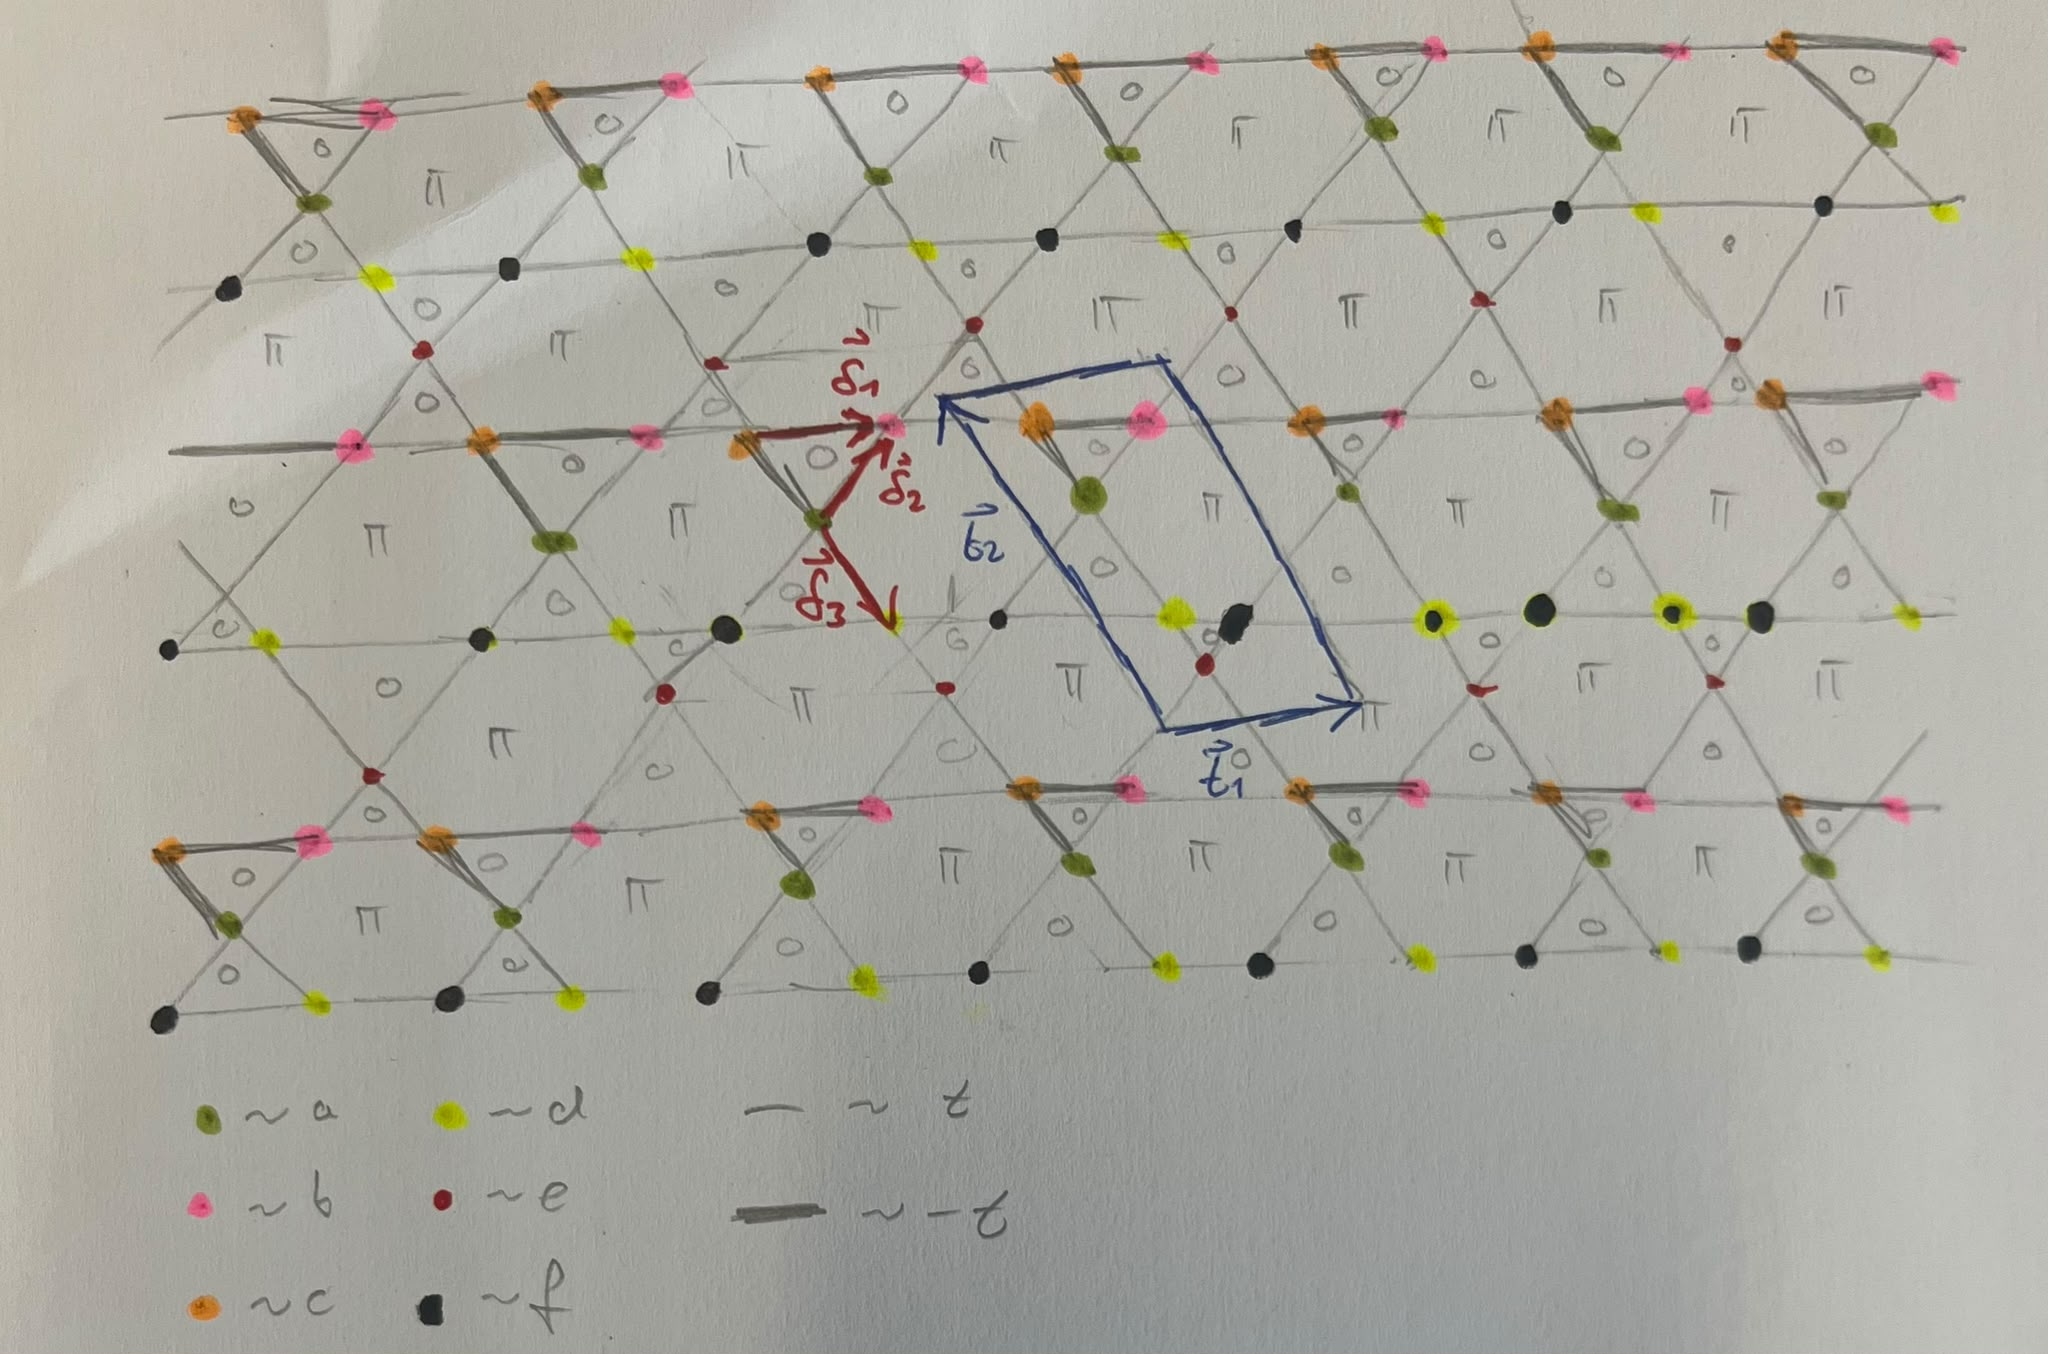
\includegraphics[width=\textwidth]{lattice-pi-flux-state.jpeg}
\end{center}

The nearest neighbour vectors remain unchanged

\begin{equation}
	\vec{\delta}_1 = 
	\begin{pmatrix}
		1 \\ 
		0
	\end{pmatrix} \quad
	\vec{\delta}_2 = \frac12
	\begin{pmatrix}
		1 \\
		\sqrt{3}
	\end{pmatrix} \quad
	\vec{\delta}_3 = \frac12 
	\begin{pmatrix}
		1 \\
		-\sqrt{3}
	\end{pmatrix}.
\end{equation}

The new primitve translations are

\begin{equation}
	\vec{t}_1 = 
	\begin{pmatrix}
		2 \\
		0
	\end{pmatrix} \quad
	\vec{t}_2 =
	\begin{pmatrix}
		-2 \\
		2\sqrt{3}
	\end{pmatrix}
\end{equation}

The real space (effective) tight-binding hamiltonian is

\begin{align}
	\begin{split}
		H = t \sum_{i\sigma}\bigg( &- a_{i\sigma}^\dagger c_{i\sigma} - c_{i\sigma}^\dagger b_{i\sigma} + b_{i\sigma}^\dagger a_{i\sigma} + a_{i\sigma}^\dagger d_{i\sigma} + d_{i\sigma}^\dagger e_{i\sigma} + e_{i\sigma}^\dagger f_{i\sigma} + f_{i\sigma}^\dagger d_{i\sigma} \\
		&+ b_{i\sigma}c_{i+t_1;\sigma} + b_{i\sigma}e_{i+t_1+t_2;\sigma} + f_{i\sigma}d_{i+t_1;\sigma} + f_{i\sigma}c_{i-t_2;\sigma} +\text{h.c.} \bigg)
	\end{split}
\end{align}

\subsubsection{Reciprocal Space}

The reciprocal lattice vectrors are 

\begin{equation}
	\vec{b}_{1} = \pi
	\begin{pmatrix}
		1 \\
		1/\sqrt{3}
	\end{pmatrix} \quad 
	\vec{b}_2 = \pi 
	\begin{pmatrix}
		0 \\
		1/\sqrt{3}
	\end{pmatrix}
\end{equation}

After a Fourier transform the $k$-space Hamiltonian reads

\begin{equation}
	H = t \sum_{q,\sigma} \Psi_{q\sigma}^\dagger 
	\begin{pmatrix}
		0 & e^{iq_2} & -e^{-iq_3} & 0 & e^{-iq_2} & e^{iq_3} \\
		e^{-iq_2} & 0 & 2i\sin(q_1) & e^{iq_2} & 0 & 0 \\
		-e^{iq_3} & -2i\sin(q_1) & 0 & e^{-iq_3} & 0 & 0 \\
		0 & e^{-iq_2} & e^{iq_3} & 0 & e^{iq_2} & e^{-iq_3} \\
		e^{iq_2} & 0 & 0 &  e^{-iq_2} & 0 & 2\cos(q_1) \\
		e^{-iq_3} & 0 & 0 & e^{iq_3} & 2\cos(q_1) & 0 
	\end{pmatrix}
	\Psi_{q\sigma},
\end{equation}

where
\begin{equation}
	\Psi_{q\sigma} = 
	\begin{pmatrix}
		a_{q\sigma} & b_{q\sigma} & c_{q\sigma} & e_{q\sigma} & f_{q\sigma} & d_{q\sigma} 
	\end{pmatrix}.
\end{equation}

\textcolor{red}{If I write this down somewhere serious, I should just label the sites differently.} \\

I used the shorthand $q_i \equiv \vec{q}\cdot\vec{\delta}_i$.

\end{document}
